\chapter{Heterogeneidade na dinâmica}
\label{cap.HetDinamica}
 
\section{Introdução}

No capítulo~\ref{cap.Heterogeneidade} foi introduzido o conceito de heterogeneidade de tamanhos de domínios, inicialmente dentro do contexto do modelo de percolação explosiva, onde essa medida, desempenhando o papel de um observável que sinaliza a ocorrência de uma transição de fase, se revelou um importante instrumento na determinação do caráter contínuo da transição observada no modelo. O sucesso do uso da heterogeneidade, nesse contexto, motivou o estudo detalhado de suas propriedades de escala, bem como a sua aplicação nos modelos de percolação de sítios e de ligações, e ainda nos modelos de Ising e Potts. Esses estudos, nos quais a heterogeneidade foi analisada em estados de equilíbrio, tornam natural o questionamento a respeito de sua possível aplicação a sistemas que se encontram fora do equilíbrio, motivando um estudo com a finalidade de tentar caracterizar suas propriedades dinâmicas, e determinar que tipo de informações a mesma poderia fornecer sobre sistemas nessas condições.

Como fatores adicionais que estimulam o estudo da heterogeneidade em sistemas que se encontram fora do equilíbrio, estão questões ainda em aberto, originadas em trabalhos sobre a dinâmica desses sistemas, e a possibilidade que essa medida possa se mostrar útil na elucidação das mesmas. Como um exemplo, temos o comportamento inesperado da distribuição de tamanhos de domínios no modelo de Potts com $q=3$, apresentado no capítulo~\ref{cap.Crescimento}, que evolui após um \textit{quench}, a partir da temperatura crítica, de uma forma compatível com a dinâmica descrita pela Eq.~(\ref{eq.dq2tTc}), embora a mesma, em princípio, seja apenas aplicável ao caso $q=2$.

O estudo das propriedades da heterogeneidade de tamanhos de domínios na dinâmica do modelo de Potts, apresentado neste trabalho, foi baseado em simulações numéricas utilizando o método de Monte Carlo, em uma rede bidimensional quadrada com condições periódicas de contorno, para diversos tamanhos de rede e três diferentes protocolos de \textit{quench}: da temperatura crítica $T_c$ para $T_c/2$, da temperatura infinita para $T_c/2$, e da temperatura infinita para $T_c$, conforme ilustrado na figura~\ref{fig.temperaturas}.

\begin{figure}[h!]
 \setlength\fboxsep{10pt}
 \setlength\fboxrule{0.5pt}
 \centering
 \fbox{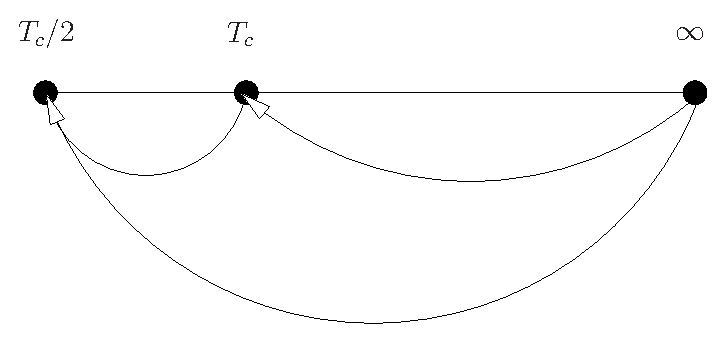
\includegraphics[width=14cm]{img/temperaturas.eps}}
 \caption{Diferentes protocolos de \textit{quench} utilizados nas simulações.}
\label{fig.temperaturas}
\end{figure}


\section{Temperatura inicial crítica e $q=2$}
\label{sec.TcQ2}

Na figura \ref{fig.het_q2_Tc_Tc2} é apresentado o gráfico da heterogeneidade ($H$) de tamanhos de domínios geométricos, para $q=2$, na rede quadrada, durante a evolução do sistema, após um \textit{quench} a partir da temperatura crítica para $T_f=T_c/2$. São apresentadas medidas para tamanhos lineares $L=32, 64, 128, 256, 512$ e $1024$. Os tempos $t$ são medidos a partir do \textit{quench}, em passos de Monte Carlo (MCs), onde cada passo corresponde a $N$ tentativas aleatórias de atualizar o estado dos spins, sendo $N$ o número total de spins na rede.

Na simulação, os spins foram inicialmente escolhidos de forma aleatória, entre os dois valores possíveis, sendo o sistema então submetido a um processo de termalização, que consistiu em permitir a evolução do mesmo, na temperatura crítica, durante um intervalo de tempo suficiente para que pudesse ser considerado em equilíbrio. O sistema foi então submetido ao \textit{quench} para a temperatura $T_f=T_c/2$, e, a partir desse ponto, a simulação da dinâmica foi feita através do algoritmo do \textit{banho térmico}~\cite{Newman}. Após a realização de determinado número de passos de Monte Carlo ($t=2^0..2^{10}$), o conjunto de domínios geométricos presentes no sistema foi determinado, através do algoritmo de Hoshen-Kopelman~\cite{HoshenKopelman}. A partir da configuração de domínios, foi produzida para cada passo uma medida da heterogeneidade de tamanhos de domínios, bem como uma medida da distribuição desses tamanhos. Para cada tempo foi feita uma média sobre até 1000 amostras.

Para simular a dinâmica do sistema durante o processo de termalização, foi empregado o algoritmo de Swendsen-Wang~\cite{SwendsenWang}. Este algoritmo é baseado na construção de aglomerados físicos, conforme descritos por Fortuin e Kasteleyn~\cite{FortuinKasteleyn} e Coniglio e Klein~\cite{ConiglioKlein}, que são então atualizados, sendo o estado de cada spin do aglomerado atualizado para um mesmo valor, entre os dois valores possíveis, escolhido de forma aleatória com igual probabilidade. Cada atualização de todos os aglomerados físicos do sistema é denominada passo de Swendsen-Wang. O número de passos necessários para que o sistema atingisse o equilíbrio na temperatura crítica foi fixado em 500 passos de Swendsen-Wang, em concordância com o protocolo descrito na Ref.~\cite{TeseMP}. A utilização de um algoritmo como o de Swendsen-Wang se justifica pelo fato de o mesmo ser consideravelmente mais eficiente que algoritmos do tipo \textit{single-flip}, como o de Metropolis e do banho térmico, nas proximidades do ponto crítico, por serem estes muito suscetíveis ao fenômeno conhecido como desaceleração crítica, ou ralentamento crítico, que torna a dinâmica do sistema extremamente lenta nessa região. No entanto, embora o algoritmo de Swendsen-Wang seja útil para levar o sistema rapidamente a um estado de equilíbrio, o que é desejável na etapa de termalização, o mesmo tem uma dinâmica não-local, o que impede a sua utilização na etapa após o \textit{quench} para $T_f=T_c/2$, onde se realizam medidas enquanto o sistema evolui fora do equilíbrio, o que explica a utilização de dois diferentes algoritmos de Monte Carlo, nas diferentes etapas da simulação. 

Observando-se o gráfico apresentado na figura \ref{fig.het_q2_Tc_Tc2}, é possível perceber que as curvas apresentam dois comportamentos distintos, visíveis para grandes tamanhos de rede. Para tempos pequenos, $H$ se mantém aproximadamente constante, enquanto que, a partir de um certo ponto, parece decair como uma lei de potência. Com o objetivo de tentar obter informações sobre o comportamento de $H$, e determinar a sua forma de escala, foi construído o gráfico apresentado na figura~\ref{fig.het_q2_Tc_Tc2_colXY}. O eixo vertical foi reescalado como $H \rightarrow HL^{-d/\tau}$. Essa forma era esperada, pelo fato de a heterogeneidade no tempo $t=0$ ser equivalente à heterogeneidade do sistema em equilíbrio, $H(t=0)=H_{\scriptstyle\rm eq}(T_c)$, cuja forma de escala foi determinada para o modelo de Ising, utilizando-se escalamento de tamanhos finitos, conforme apresentado no capítulo~\ref{cap.Heterogeneidade}, e ilustrado pelo colapso obtido na figura~\ref{fig.IsingHCol}. Nessa expressão, $d$ é a dimensão do sistema e $\tau$ é um expoente que caracteriza o tamanho dos domínios. Utilizou-se $\tau = 187/91$, que é o valor exato para domínios geométricos no modelo de Ising, para a temperatura crítica~\cite{PRLJeferson,PREJeferson}. O eixo horizontal foi reescalado como $t \rightarrow t/L$. Conforme pode ser observado na figura~\ref{fig.het_q2_Tc_Tc2_colXY}, as curvas de $H$ parecem convergir assintoticamente para uma mesma reta, com o aumento do tamanho do sistema, indicando um comportamento do tipo lei de potência no limite termodinâmico. A justificativa para o desvio da lei de potência parece residir no fato que sistemas menores chegam antes a um estado magnetizado, com domínios associados às flutuações térmicas, o que faz com que $H$ atinja um valor estacionário. No limite termodinâmico, o tempo para cair em um estado magnetizado diverge, e se esperaria a convergência de $H$ para a lei de potência. A linha reta pontilhada, apresentada no gráfico, tem uma declividade aproximadamente igual a $-0.82$, determinada através de ajuste aos dados da curva de $H$ para $L=1024$. No entanto, serão necessários resultados obtidos com sistemas maiores, para que se possa obter um valor próximo ao esperado para o expoente no limite termodinâmico.

\begin{figure}[p]
 \centering
 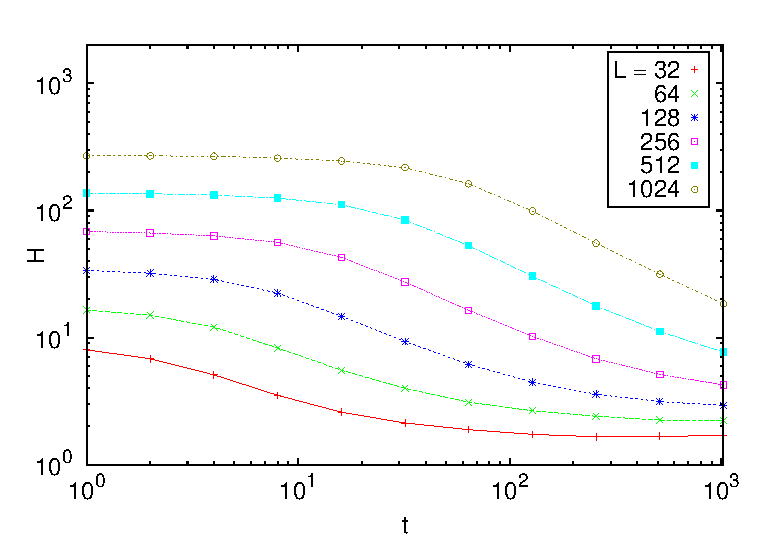
\includegraphics[width=14cm]{fig/het_q2_Tc_Tc2.eps}
 \caption{Variação da heterogeneidade de tamanhos de domínios geométricos para o modelo de Ising na rede quadrada, após um \textit{quench} de $T_0=T_c$ para $T_f=T_c/2$, para diferentes valores de $L$.}
\label{fig.het_q2_Tc_Tc2}
\vspace{8mm}
 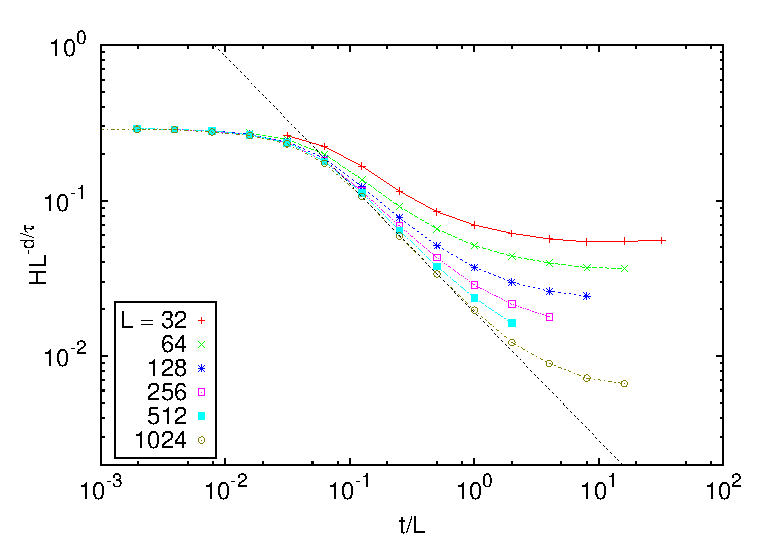
\includegraphics[width=14cm]{fig/het_q2_Tc_Tc2_colXY.eps}
 \caption{Análise de escala da heterogeneidade de tamanhos de domínios geométricos para o modelo de Ising na rede quadrada, após um \textit{quench} de $T_0=T_c$ para $T_f=T_c/2$. Os dados são os mesmos utilizados na figura~\ref{fig.het_q2_Tc_Tc2}. A linha reta pontilhada tem declividade $-0.82$.}
\label{fig.het_q2_Tc_Tc2_colXY}
\end{figure}


\section{Temperatura inicial infinita e $q=2$}
\label{sec.TinfQ2}

Na figura \ref{fig.het_q2_Tinf_Tc2} é apresentado o gráfico da heterogeneidade de tamanhos de domínios geométricos, para $q=2$, após um \textit{quench} a partir da temperatura infinita para $T_f=T_c/2$. Como no caso anterior, são apresentadas medidas para tamanhos lineares $L=32, 64, 128, 256, 512$ e $1024$. A temperatura inicial infinita equivale a um estado onde os spins estão totalmente descorrelacionados, sendo cada um dos mesmos escolhido de forma aleatória entre os dois valores possíveis. A simulação da dinâmica, após o \textit{quench}, foi feita através do algoritmo do banho térmico, sendo as medidas realizadas exatamente como descrito para o caso com temperatura inicial crítica.

Assim como apresentado na seção~\ref{sec.TcQ2}, foi feita uma tentativa de se determinar a forma de escala de $H$ neste caso, sendo o eixo vertical reescalado como $H \rightarrow HL^{-d/\tau}$ e o horizontal como $t \rightarrow t/L$. Utilizou-se $\tau = 379/187$, que é o valor exato para domínios geométricos no modelo de Ising, para a temperatura infinita~\cite{PRLJeferson,PREJeferson}. O resultado pode ser observado na figura~\ref{fig.het_q2_Tinf_Tc2_colXY}. Mais uma vez, parece que temos um colapso progressivo das curvas, com uma convergência assintótica para uma lei de potência, com o aumento do tamanho do sistema. Percebe-se ainda, no comportamento de $H$, um pequeno decaimento inicial, atribuído ao fato de que neste caso, em um ou dois passos de Monte Carlo, o sistema atinge o estado crítico percolativo~\cite{PRLJeferson}, o que leva ao aparecimento de um domínio percolante, que ocupa uma fração considerável da rede, diminuindo a quantidade e diversidade dos domínios (apesar da distribuição ficar mais larga). A linha reta pontilhada, apresentada no gráfico, tem uma declividade aproximadamente igual a $-0.85$, determinada através de ajuste aos dados da curva de $H$ para $L=1024$.

\begin{figure}[p]
 \centering
 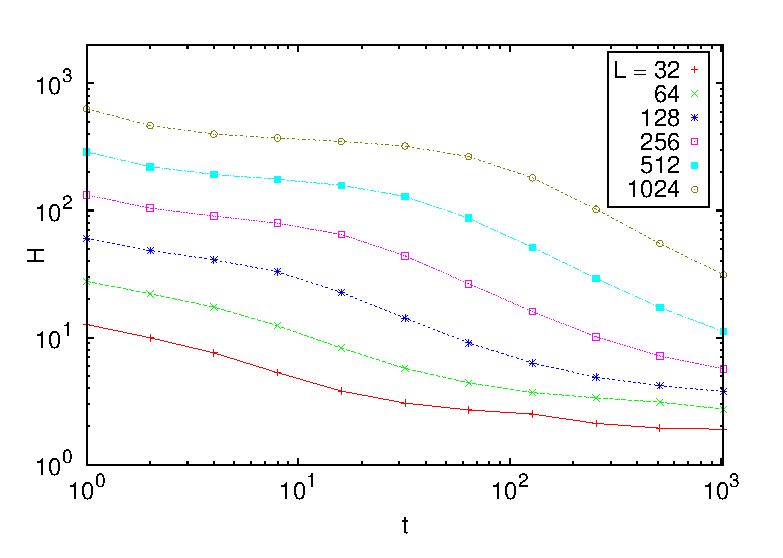
\includegraphics[width=14cm]{fig/het_q2_Tinf_Tc2.eps}
 \caption{Variação da heterogeneidade de tamanhos de domínios geométricos para o modelo de Ising na rede quadrada, após um \textit{quench} de $T_0\rightarrow \infty$ para $T_f=T_c/2$, para diferentes valores de $L$.}
\label{fig.het_q2_Tinf_Tc2}
\vspace{8mm}
 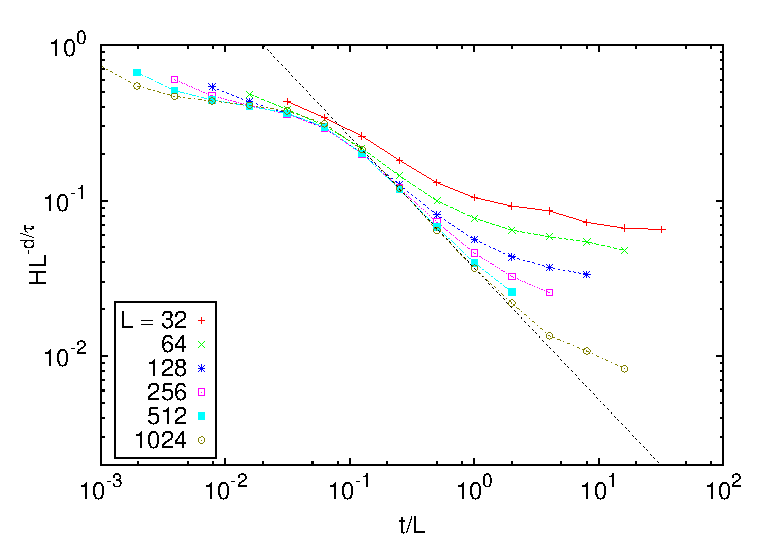
\includegraphics[width=14cm]{fig/het_q2_Tinf_Tc2_colXY.eps}
 \caption{Análise de escala da heterogeneidade de tamanhos de domínios geométricos para o modelo de Ising na rede quadrada, após um \textit{quench} de $T_0\rightarrow \infty$ para $T_f=T_c/2$. Os dados são os mesmos utilizados na figura~\ref{fig.het_q2_Tinf_Tc2}. A linha reta pontilhada tem declividade $-0.85$.}
\label{fig.het_q2_Tinf_Tc2_colXY}
\end{figure}


\section{Temperatura inicial crítica e $q=3$}
\label{sec.TcQ3}

Na figura \ref{fig.het_q3_Tc_Tc2} é apresentado o gráfico da heterogeneidade de tamanhos de domínios geométricos, para $q=3$, na rede quadrada, durante a evolução do sistema, após um \textit{quench} a partir da temperatura crítica para $T_f=T_c/2$. São apresentadas medidas para tamanhos lineares $L=32, 64, 128, 256, 512$ e $1024$. O procedimento adotado na simulação foi análogo ao apresentado na seção \ref{sec.TcQ2}.

Mais uma vez, foi feita uma tentativa de se determinar a forma de escala de $H$, sendo o eixo vertical reescalado como $H \rightarrow HL^{-d/\tau}$ e o horizontal como $t \rightarrow t/L$. Utilizou-se $\tau = 187/91$, que é o valor exato para domínios geométricos no modelo de Ising, para a temperatura crítica~\cite{PRLJeferson,PREJeferson}. Para domínios geométricos no modelo de Potts, com $q=3$, o valor de $\tau$ não é conhecido exatamente, mas é bastante próximo ao encontrado para o modelo de Ising~\cite{LoureiroPRE}. O resultado pode ser observado na figura~\ref{fig.het_q3_Tc_Tc2_colXY}. Novamente, as curvas de $H$ parecem convergir assintoticamente para uma mesma reta, com o aumento do tamanho do sistema, indicando um comportamento do tipo lei de potência no limite termodinâmico. A linha reta pontilhada, apresentada no gráfico, tem uma declividade aproximadamente igual a $-0.82$, determinada através de ajuste aos dados da curva de $H$ para $L=1024$.

\begin{figure}[p]
 \centering
 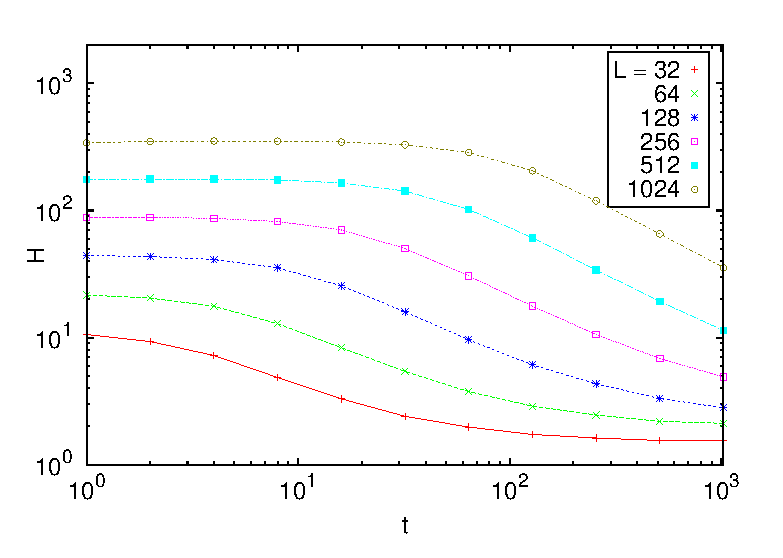
\includegraphics[width=14cm]{fig/het_q3_Tc_Tc2.eps}
 \caption{Variação da heterogeneidade de tamanhos de domínios geométricos para o modelo de Potts na rede quadrada, com $q=3$, após um \textit{quench} de $T_0=T_c$ para $T_f=T_c/2$, para diferentes valores de $L$.}
\label{fig.het_q3_Tc_Tc2}
\vspace{8mm}
 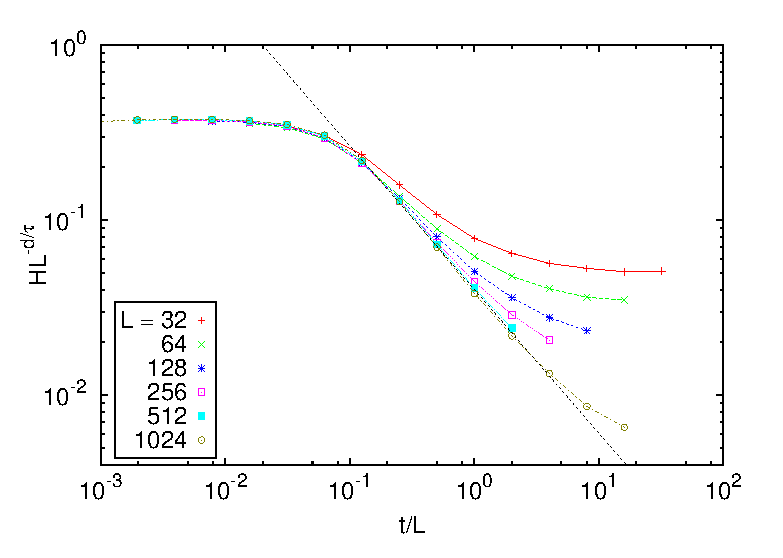
\includegraphics[width=14cm]{fig/het_q3_Tc_Tc2_colXY.eps}
 \caption{Análise de escala da heterogeneidade de tamanhos de domínios geométricos para o modelo de Potts na rede quadrada, com $q=3$, após um \textit{quench} de $T_0=T_c$ para $T_f=T_c/2$. Os dados são os mesmos utilizados na figura~\ref{fig.het_q3_Tc_Tc2}. A linha reta pontilhada tem declividade $-0.82$.}
\label{fig.het_q3_Tc_Tc2_colXY}
\end{figure}


\section{Temperatura inicial infinita e $q=3$}
\label{sec.TinfQ3}

Na figura \ref{fig.het_q3_Tinf_Tc2} é apresentado o gráfico da heterogeneidade de tamanhos de domínios geométricos, para $q=3$, na rede quadrada, durante a evolução do sistema, após um \textit{quench} a partir da temperatura infinita para $T_f=T_c/2$. São apresentadas medidas para tamanhos lineares $L=32, 64, 128, 256, 512$ e $1024$. O procedimento adotado na simulação foi análogo ao apresentado na seção~\ref{sec.TinfQ2}. Em relação aos casos anteriores, percebe-se uma diferença qualitativa: enquanto nos demais casos as curvas parecem ser estritamente decrescentes, neste as curvas claramente possuem um ponto máximo. Com o objetivo de se obter mais informações sobre esse máximo, é apresentado na figura~\ref{fig.hetevlin_q3_Tinf_Tc2} um gráfico linear, no qual $H$ foi medido para todos os passos de Monte Carlo, o que facilita a determinação das posições onde ocorrem os máximos nas curvas (indicados por segmentos de reta verticais). Na figura~\ref{fig.areasev_q3_L512_Tinf_Tc2}, observamos ainda o gráfico das distribuições para este caso, com $L=512$, utilizando os mesmos dados usados na construção da figura~\ref{fig.hetevlin_q3_Tinf_Tc2}, com a curva para o tempo em que ocorre o máximo valor de $H$ em destaque. Aparentemente, não é possível perceber através da curva da distribuição qualquer particularidade que indique um correspondente máximo na heterogeneidade.

\begin{figure}[p]
 \centering
 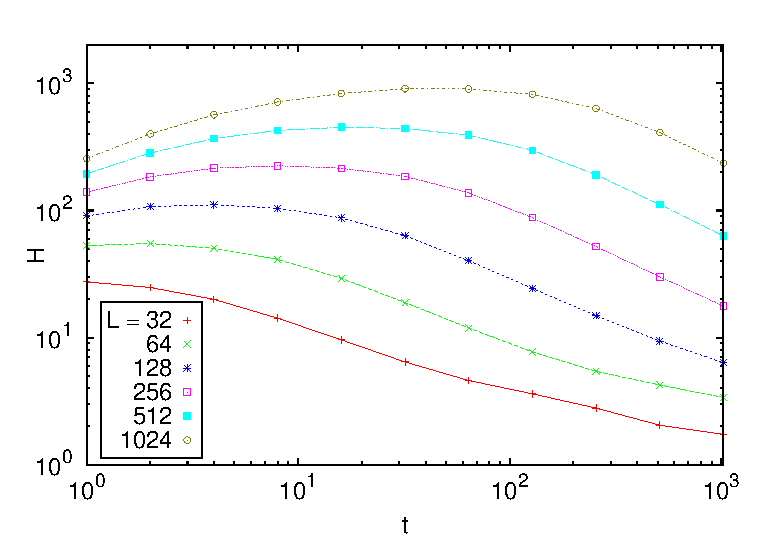
\includegraphics[width=14cm]{fig/het_q3_Tinf_Tc2.eps}
 \caption{Variação da heterogeneidade de tamanhos de domínios geométricos para o modelo de Potts na rede quadrada, com $q=3$, após um \textit{quench} de $T_0\rightarrow \infty$ para $T_f=T_c/2$, para diferentes valores de $L$.}
\label{fig.het_q3_Tinf_Tc2}
\vspace{8mm}
 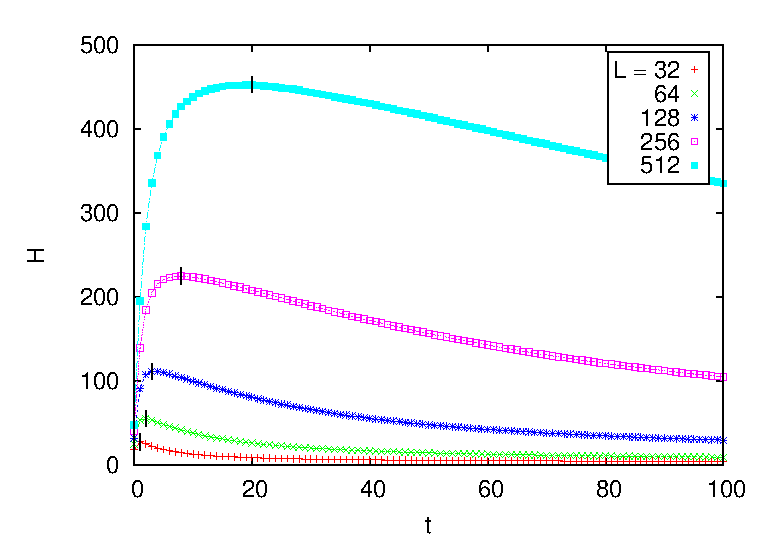
\includegraphics[width=14cm]{fig/hetevlin_q3_Tinf_Tc2.eps}
 \caption{Gráfico linear da heterogeneidade de tamanhos de domínios geométricos para o modelo de Potts na rede quadrada, com $q=3$, após um \textit{quench} de $T_0\rightarrow \infty$ para $T_f=T_c/2$, para diferentes valores de $L$, com a posição aproximada dos máximos indicada por segmentos de reta verticais.}
\label{fig.hetevlin_q3_Tinf_Tc2}
\end{figure}

Como nos casos anteriores, foi feita uma tentativa de se determinar a forma de escala de $H$, sendo o eixo vertical reescalado como $H \rightarrow HL^{-d/\tau}$ e o horizontal como $t \rightarrow t/L$. Utilizou-se $\tau = 379/187$, que é o valor exato para domínios geométricos no modelo de Ising, para a temperatura infinita~\cite{PRLJeferson,PREJeferson}, como uma aproximação para o caso com $q=3$, justificada pela proximidade dos valores~\cite{LoureiroPRE}. O resultado pode ser observado na figura~\ref{fig.het_q3_Tinf_Tc2_colXY}. Mais uma vez, parece que temos um colapso progressivo das curvas, com uma convergência assintótica para uma lei de potência, com o aumento do tamanho do sistema. A linha reta pontilhada, apresentada no gráfico, tem uma declividade aproximadamente igual a $-0.87$, determinada através de ajuste aos dados da curva de $H$ para $L=1024$.

\begin{figure}[p]
 \centering
 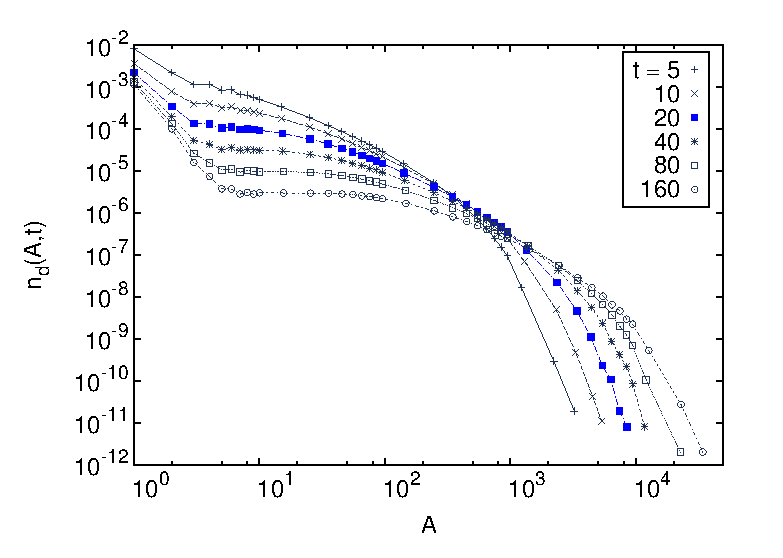
\includegraphics[width=14cm]{fig/areasev_q3_L512_Tinf_Tc2.eps}
 \caption{Distribuições de tamanhos de domínios geométricos para o modelo de Potts na rede quadrada, com $q=3$ e $L=512$, após um \textit{quench} de $T_0\rightarrow \infty$ para $T_f=T_c/2$, para diferentes tempos, utilizando os mesmos dados usados na construção da figura~\ref{fig.hetevlin_q3_Tinf_Tc2}, com a curva para o tempo $t=20$, em que ocorre o máximo valor de $H$, em destaque.}
\label{fig.areasev_q3_L512_Tinf_Tc2}
\vspace{8mm}
 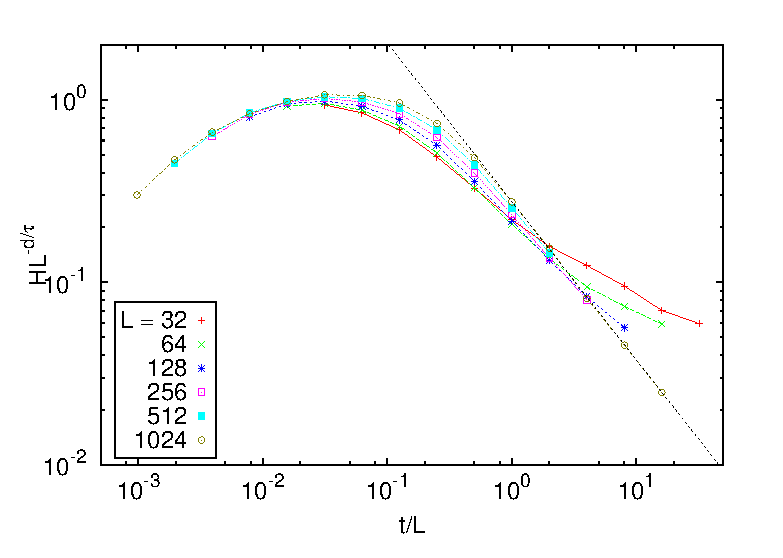
\includegraphics[width=14cm]{fig/het_q3_Tinf_Tc2_colXY.eps}
 \caption{Análise de escala da heterogeneidade de tamanhos de domínios geométricos para o modelo de Potts na rede quadrada, com $q=3$, após um \textit{quench} de $T_0\rightarrow \infty$ para $T_f=T_c/2$. Os dados são os mesmos utilizados na figura~\ref{fig.het_q3_Tinf_Tc2}. A linha reta pontilhada tem declividade $-0.87$.}
\label{fig.het_q3_Tinf_Tc2_colXY}
\end{figure}


\section{Temperatura inicial infinita e temperatura final crítica}

Com a finalidade de verificar se o comportamento caracterizado pela presença de um máximo na variação da heterogeneidade ocorre também em outros protocolos de \textit{quench} que partem da temperatura infinita, foram realizadas simulações onde o \textit{quench} foi feito de $T_0\rightarrow \infty$ para $T_f=T_c$, para $q=2$ e $q=3$. A escolha desse particular protocolo foi sugerida pelo recente trabalho de Blanchard \textit{et al}~\cite{BlanchardCugliandoloPicco}, no qual o mesmo foi utilizado no estudo de propriedades dinâmicas do modelo de Ising, embora com diferentes tipos de domínios ou geometrias de rede. O resultado obtido pode ser observado na figura~\ref{fig.het_L1024_Tc_lines}, onde se pode perceber a presença de um máximo na curva de $H$, para $q=3$. As linhas retas pontilhadas, apresentadas no gráfico, são paralelas, com uma declividade aproximadamente igual a $-0.21$, determinada através de ajuste aos dados obtidos para $q=3$. Entretanto, para que seja possível verificar a forma de convergência assintótica das curvas, e ainda, no caso de uma lei de potência, determinar o valor do expoente, serão necessárias simulações adicionais, para diferentes tamanhos de rede, bem como uma análise do colapso dos dados obtidos.

\begin{figure}[h!]
 \centering
 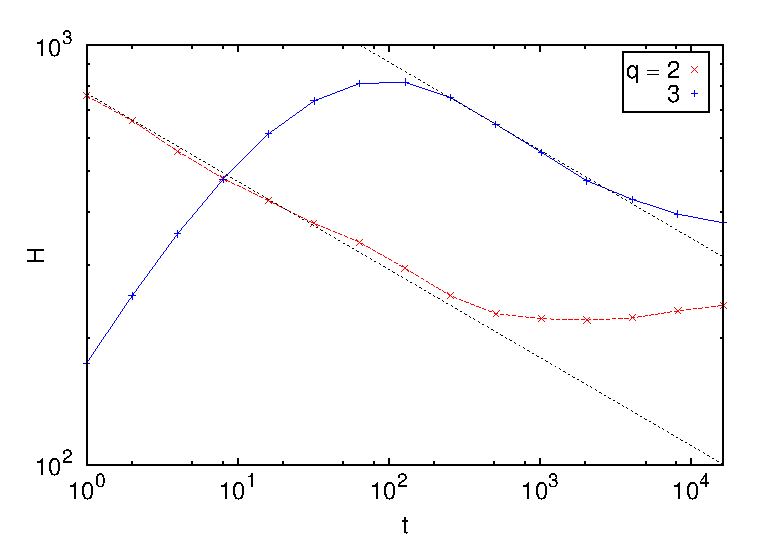
\includegraphics[width=14cm]{fig/het_L1024_Tc_lines.eps}
 \caption{Variação da heterogeneidade de tamanhos de domínios geométricos para o modelo de Potts na rede quadrada, para $q=2$ e $q=3$, após um \textit{quench} de $T_0\rightarrow \infty$ para $T_f=T_c$, para $L=1024$. As linhas retas pontilhadas são paralelas, com declividade $-0.21$.}
\label{fig.het_L1024_Tc_lines}
\end{figure}


\section{Comparações entre diferentes protocolos de \textit{quench}}

As diferenças no comportamento dinâmico da heterogeneidade, para os diferentes protocolos de \textit{quench} estudados, tornam-se mais perceptíveis quando as curvas obtidas em cada caso, para um mesmo tamanho de rede, são apresentadas no mesmo gráfico, como pode ser observado na figura~\ref{fig.het_L1024_Tc2_lines}, gerada para $L=1024$. Percebe-se claramente a diferença qualitativa, já mencionada, da existência de um máximo na curva, no caso em que $q=3$ e $T_0\rightarrow \infty$, contrastando com o comportamento estritamente decrescente nos demais casos. Apesar dessa diferença, pode-se observar que todas as curvas parecem convergir, para tempos grandes, para retas com aproximadamente a mesma declividade, sugerindo um comportamento do tipo lei de potência, com o mesmo expoente para todos os casos. As linhas retas pontilhadas, apresentadas no gráfico, são todas paralelas, com uma declividade aproximadamente igual a $-0.86$, determinada através de ajuste aos dados obtidos para $q=3$ e $T_0\rightarrow \infty$. Essas retas, no entanto, são indicativas do comportamento para esse particular tamanho de rede, não necessariamente refletindo o que se obteria no limite termodinâmico. Para se reduzir o erro na determinação do valor do expoente, serão necessárias simulações adicionais, para permitir uma análise de escala com tamanhos de rede maiores.

Nota-se ainda que as curvas para os casos onde $q=2$, $T_0\rightarrow \infty$, e $q=3$, $T_0=T_c$, estão praticamente colapsadas, enquanto que no caso onde $q=2$ e $T_0=T_c$, embora a curva tenha uma forma semelhante, está deslocada em relação às demais. Pode-se obter um colapso aproximado desta última curva sobre as primeiras, multiplicando-se o valor de $H$ por um fator aproximadamente igual a $2$. Atribuímos esse comportamento ao fator $2$ que aparece na expressão da distribuição para o caso $q=2$, $T_0\rightarrow \infty$, mas não no caso $q=2$, $T_0=T_c$, conforme pode ser observado nas Eq.~(\ref{eq.dq2tTinf}) e (\ref{eq.dq2tTc}), e também a um fator 2 que aparece na distribuição determinada heuristicamente por Loureiro \textit{et al}, que se ajusta aos dados obtidos para $q=3$~\cite{LoureiroPRE}. Desta maneira, ao aumentar a probabilidade de uma determinada área na distribuição, aumenta sua probabilidade de aparecer em uma amostra e contribuir para o valor de $H$.

O caso onde $q=3$ e $T_0\rightarrow \infty$, dentre os aqui estudados, é o único a não apresentar uma grande cauda na distribuição, conforme pode ser observado na figura~\ref{fig.AreasCol}. Esperaríamos, em princípio, que o mesmo apresentasse valores de $H$ menores que nos demais casos. Entretanto, se verifica que ocorre o oposto. Como justificativa para esse comportamento, parece estar o fato que neste caso em geral não aparecem domínios percolantes durante o intervalo de tempo considerado, por estar a probabilidade associada a cada variedade de spin, na distribuição aleatória inicial ($1/3$), distante do valor da densidade crítica do modelo de percolação aleatória. Assim, para cada amostra do sistema, neste caso, podem aparecer um grande número de domínios, com uma grande variedade de tamanhos. Já nos demais casos estudados, há uma grande probabilidade de existirem domínios percolantes, seja pelo fato de a configuração inicial do sistema não ter temperatura infinita, estando os spins correlacionados, ou, para o caso onde $q=2$ e $T_0\rightarrow \infty$, pela proximidade da probabilidade associada a cada variedade de spin na distribuição aleatória inicial ($1/2$) com a densidade crítica do modelo de percolação aleatória $\rho_c \sim 0.59$~\cite{PRLJeferson}. Assim, para configurações com um ou mais domínios percolantes ocupando a maior parte do sistema, resta uma pequena área a ser ocupada por domínios menores, levando a uma variedade de tamanhos de domínios consideravelmente menor.

\begin{figure}[h!]
 \centering
 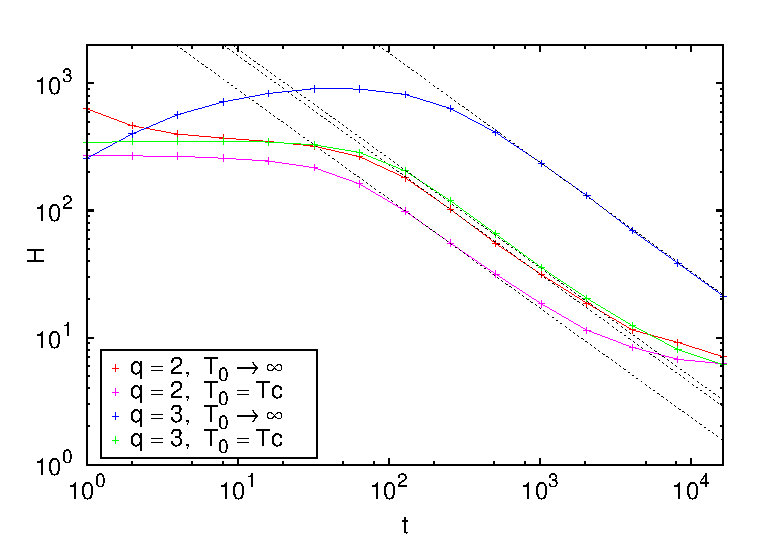
\includegraphics[width=14cm]{fig/het_L1024_Tc2_lines.eps}
 \caption{Variação da heterogeneidade de tamanhos de domínios geométricos para o modelo de Potts na rede quadrada, para diferentes valores de $q$ e temperaturas iniciais, para $L=1024$ e $T_f=T_c/2$. As linhas retas pontilhadas são todas paralelas, com declividade $-0.86$.}
\label{fig.het_L1024_Tc2_lines}
\end{figure}

